\section{新的开始}

从本科时期开始接触代码后,我便一直希望能够进行自己的项目开发,日常也喜欢写一些个人小程序自娱自乐,
因为一直对游戏较为感兴趣,因此初期希望研究并开发类似Unity的游戏引擎。
困于本科时期知识基础的薄弱,以及相关开发经验的缺乏,四年间都只做过一些较小的个人项目,
知识体系尚未形成一个较为系统的架构,没有将个人的思想融入到项目中实现。\\

研究生阶段,为了能够对读研生涯进行记录,我开始了这个项目的设计。
但是由于毕业与工作的压力,之前的文章写了部分就暂时搁浅了,而现在终于有时间来继续推进。
我的目标是将此项目作为一个完整的系统,搜集资料后按照个人的想法进行设计和实现,
不仅能够锻炼提升个人水平,还能够锻炼阅读与其他能力。
同时,这个系列的文章不仅是我个人学习过程的笔记,也将作为后续编写类似程序的相关参考,
并在这之中提出一些我个人的想法来抛砖引玉,得到他人的指导或同好的学习与分享。
最后希望通过此项目对相关领域做出一些微薄的贡献。\\

本文使用\LaTeX{}编写。

\maketitle
\section{初步的写作计划}

此项目聚焦于跨平台3D引擎的设计开发,从零开始搭建一个3D引擎用于渲染3D场景,
以及支持脚本及AI的场景内物体互动,使其具有成为仿真环境的可能性。
本项目模仿游戏引擎进行模块划分,一个游戏引擎由许多模块组成,
每个模块具有相对独立的功能,参考《游戏引擎架构》的内容,本文章将按照以下几个部分设计介绍。
当然也有部分章节可能脱离主线,介绍一些额外的内容。\\

本笔记主要参考的内容出自大名鼎鼎的Game Engine Architecture的引擎架构:
\begin{figure}[H]
\centering
%\begin{minipage}{0.1\textwidth}
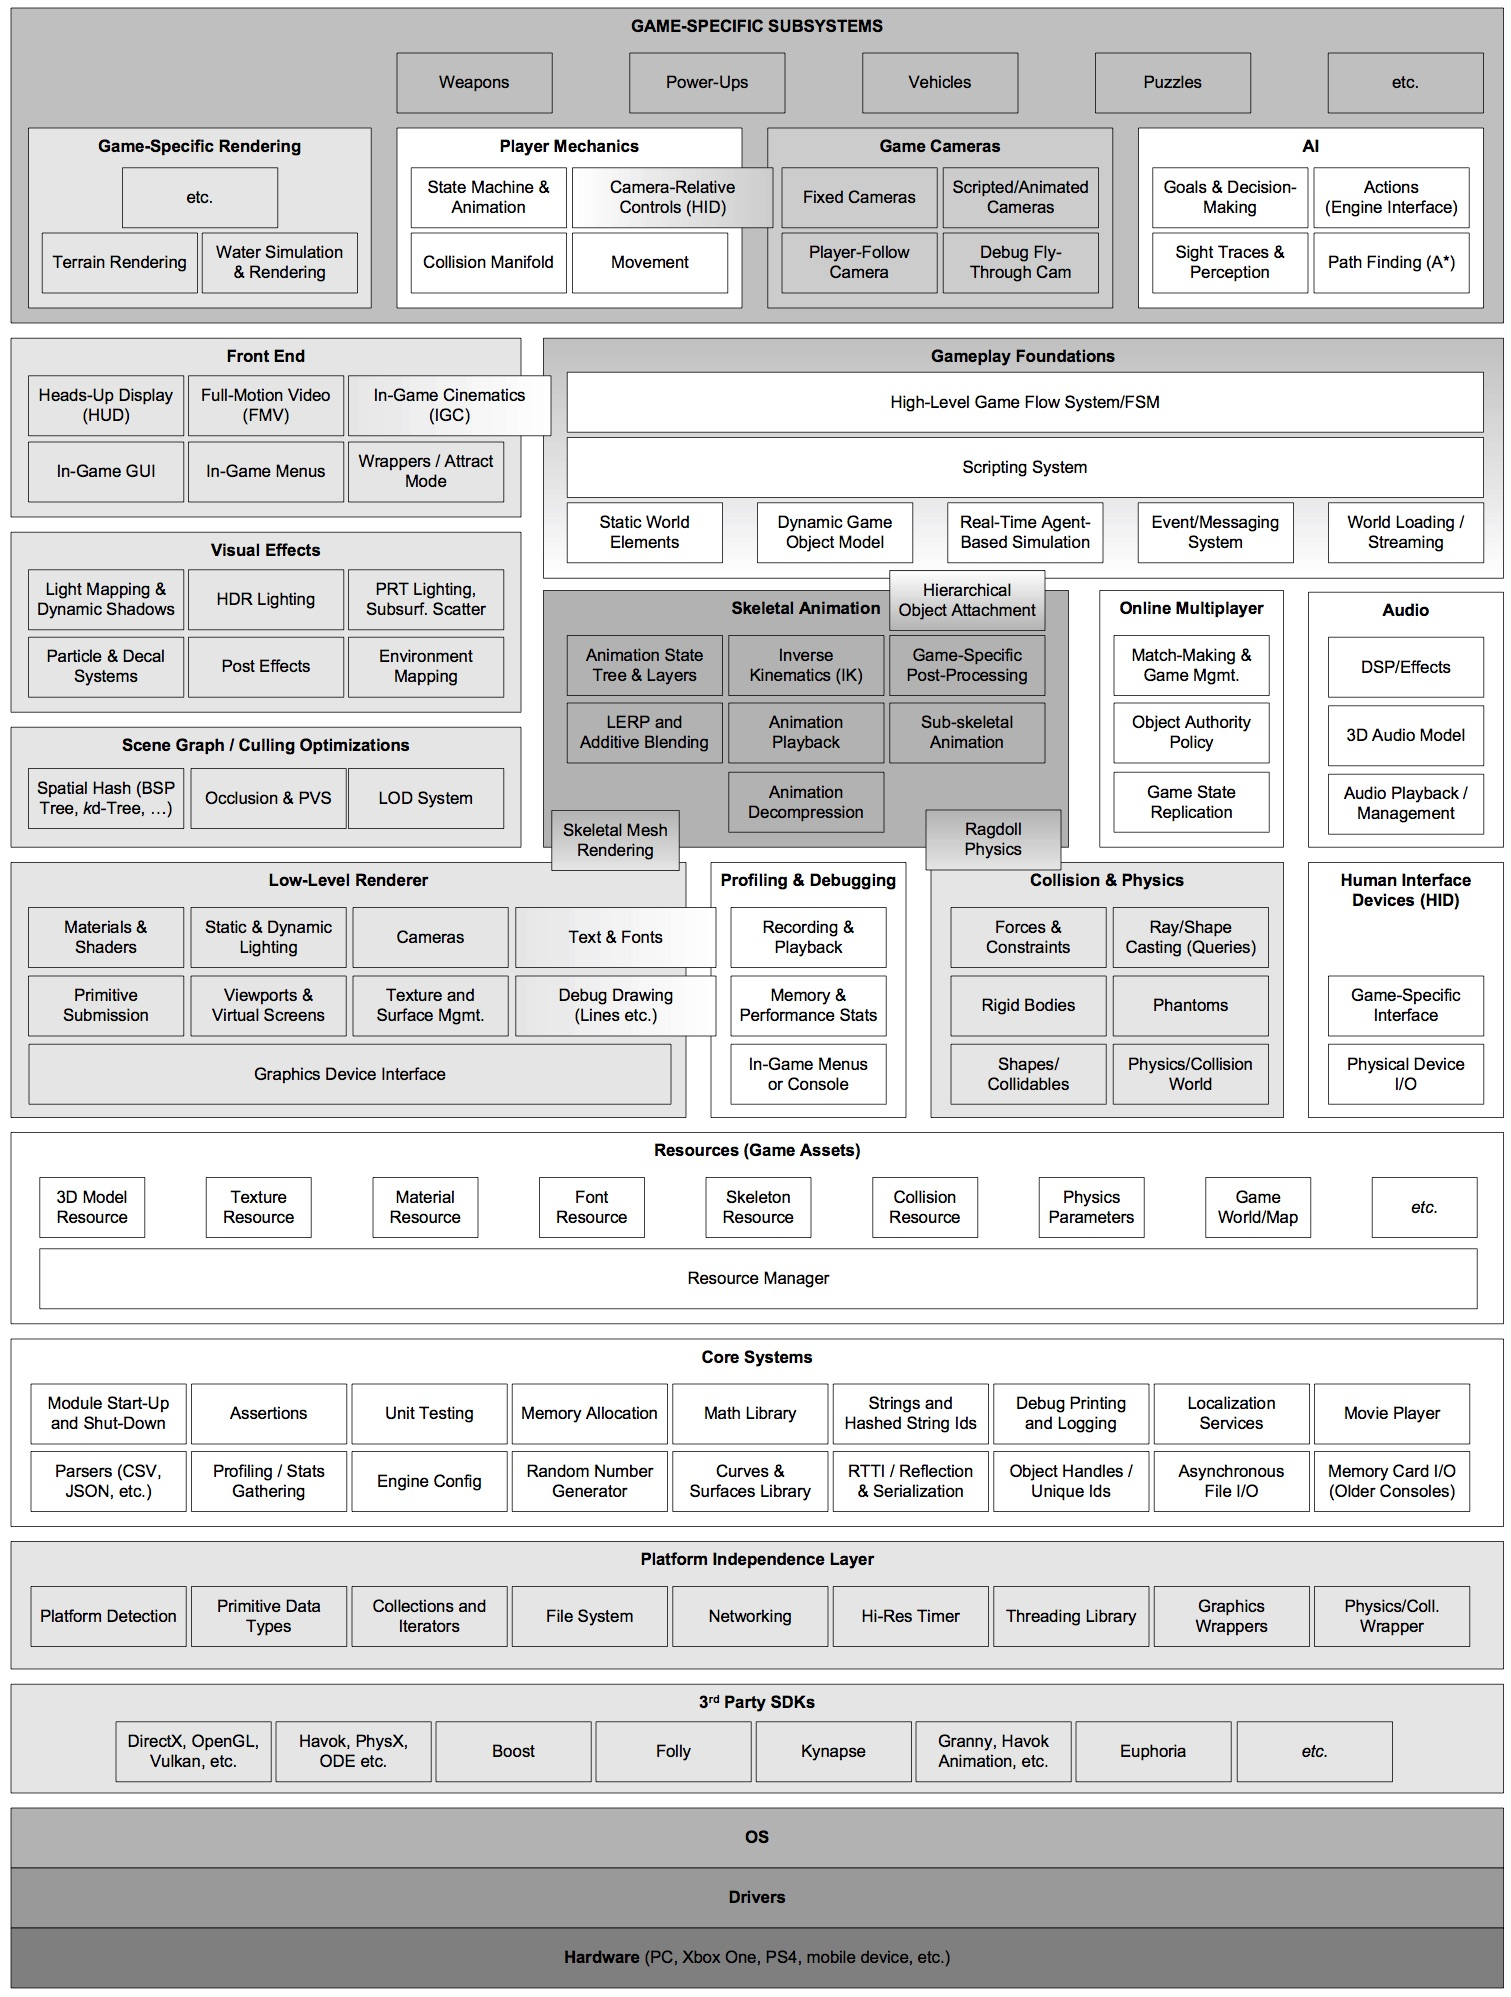
\includegraphics[center, width=0.25\textwidth]{chapter00/fig-runtime-arch.jpeg}
\caption{引擎架构图}
%\end{minipage}
\end{figure}

\maketitle
\subsection{基础系统}

这个部分用于介绍引擎底层系统的设计,作为学习的必要过程,本项目中将跟随开发进度不断修改引擎底层结构的设计。许多基础的数据结构与算法也会出现在本节。

\maketitle
\subsection{数学与几何}

随后的渲染与物理部分,都与数学紧密相关。数学构成了渲染与物理模块的基石。本节主要介绍一些基本的数学内容,作为后续部分的基础。

\maketitle
\subsection{渲染系统}

为了能够展示场景的运行效果,需要有直观的方式展现内容,3D渲染就是最好的方式。这个部分主要介绍渲染的相关内容,包括一个软渲染器以及对应的GPU版本渲染器。

\maketitle
\subsection{物理系统}

本节展示一个简单的物理仿真模块,用于刚体碰撞与刚体动力学仿真。为了引擎具有物理仿真的基础功能,也为了更好的表达引擎之中的交互,引入了物理模块作为底层。

\maketitle
\subsection{场景管理系统}

这个部分用于介绍较为大型的场景优化所需的场景管理模块的相关内容。

\maketitle
\subsection{脚本及AI系统}

本节主要介绍如何集成一个脚本系统,与场景部分相结合。由脚本系统的功能扩展AI的功能。
